\begin{lstlisting}
p110 8(1)(2)(4)
\end{lstlisting}
\begin{exercise}
\begin{figure}[H]
\centering
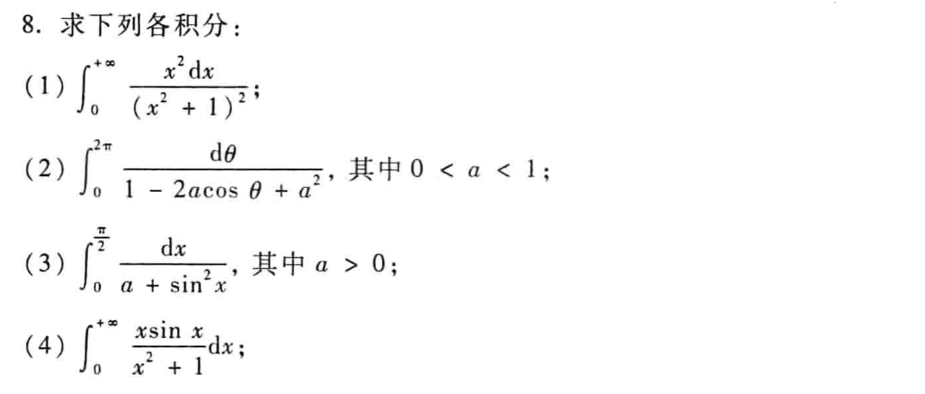
\includegraphics[width=\textwidth]{hw10-2025050521.png}
% \caption{}
\label{}
\end{figure}
\end{exercise}
(1)
Let
\[
f(z)=\frac{z^2}{(z^2+1)^2}=\frac{z^2}{(z+i)^2(z-i)^2}
\]
Consider the toy contour
\begin{figure}[H]
\centering
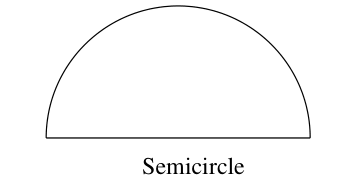
\includegraphics[width=\textwidth]{2-hw10-2025050521.png}
% \caption{}
\label{}
\end{figure}
We have
\begin{equation}
\begin{aligned}
\int_{-R}^{R} +\int_{\gamma^{+}_{R}}f(z) \, \mathrm{d}z & =2\pi i \cdot\mathrm{res}_{i}f=2\pi i\cdot \lim_{ z \to i }\frac{\mathrm{d}}{\mathrm{d}z} \frac{1}{1!} (z-i)^2f(z) \\
 & =2\pi i\cdot \lim_{ z \to i } \frac{\mathrm{d}}{\mathrm{d}z} \left( \frac{z^2}{(z+i)^2} \right) \\
 & =2\pi i\cdot \lim_{ z \to i } \left( \frac{2z}{(z+i)^2}-\frac{2z^2}{(z+i)^{3}} \right)  \\
 & =2\pi i\cdot \lim_{ z \to i } \left( -\frac{i}{4}  \right) \\
 & =\frac{\pi}{2}
\end{aligned}
\label{e8496f}
\end{equation}

On $\gamma^{+}_{R}$,
\[
\left\lvert  \int_{\gamma_{R}^{+}}^{} f(z) \, \mathrm{d}z   \right\rvert \leq \int_{\gamma_{R}^{+}}^{} \lvert f(z) \rvert \, \mathrm{d}z  =\int_{\gamma_{R}^{+}}^{} \frac{\lvert z^2 \rvert }{\lvert z^2+1 \rvert ^2 } \, \mathrm{d}z\leq \frac{R^2}{(R^2-1)^2}\cdot \pi R\to0\quad \text{as }R\to \infty
\]
Let $R\to \infty$ in \cref{e8496f}, then
\[
\int_{-\infty}^{\infty} f(z) \, \mathrm{d}z =\frac{\pi }{2}
\]
Hence
\[
\int_{0}^{\infty} f(x) \, \mathrm{d}x =\frac{1}{2}\int_{-\infty}^{\infty} f(z) \, \mathrm{d}z =\frac{\pi }{4}
\]
(2)
\[
I=\oint_{|z|=1} \frac{1}{1-2 a\left(\frac{z+z^{-1}}{2}\right)+a^2} \frac{\mathrm{~d} z}{i z}=\frac{i}{a} \oint_{|z|=1} \underbrace{ \frac{1}{z^2-\left(\frac{1+a^2}{a}\right) z+1} }_{ \eqqcolon f(z) } \mathrm{~d} z
\]
The singularities are $\frac{1}{a}$ and $a$. Since $a\in(0,1)$, then
\[
I=\frac{i}{a}\cdot2\pi i\cdot \mathrm{res}_{a}f=\frac{i}{a}\cdot2\pi i\cdot \lim_{ z \to a } (z-a)f(z)=\frac{i}{a}\cdot2\pi i\cdot\frac{1}{a-\frac{1}{a}}=\frac{2\pi }{1-a^2}
\]
(4)
\[
\int_{0}^{+\infty} \frac{x\sin x}{x^2+1} \, \mathrm{d}x =\frac{1}{2}\int_{-\infty}^{\infty} \frac{x\sin x}{x^2+1} \, \mathrm{d}x =\frac{1}{2i}\int_{-\infty}^{\infty} \frac{xe^{ ix }}{x^2+1} \, \mathrm{d}x 
\]
Let
\[
f(z)=\frac{ze^{ iz }}{z^2+1}=\frac{ze^{ iz }}{(z-i)(z+i)}
\]
Consider the toy contour, an indented semicircle in the upper plane.
\begin{equation}
\int_{-\infty}^{\infty} +\int_{\gamma^{+}_{R}}^{}  f(z) \, \mathrm{d}z= 2\pi i\cdot \mathrm{res}_{i}f=2\pi i\cdot \lim_{ z \to i } (z-i)f(z)=2\pi i\cdot\frac{ie^{ -1 }}{2i}=\frac{i\pi}{e}
\label{11089d}
\end{equation}

On $\gamma^{+}_{R}$,
\[
\left\lvert  \int_{\gamma^{+}_{R}}^{} f(z) \, \mathrm{d}z   \right\rvert \leq \int_{\gamma^{+}_{R}}^{} \lvert f(z) \rvert  \, \lvert \mathrm{d}z \rvert  =\int_{0}^{\pi} \frac{R\cdot e^{ -R \sin\theta }}{\lvert R e^{ i\theta }-i \rvert \cdot \lvert R e^{ i\theta }+i \rvert } R \, \mathrm{d}\theta\leq C\cdot e^{ -R\sin\theta }\to0\quad \text{as }R\to \infty
\]
where $\theta\in(0,\pi)$, thus $\sin\theta>0$.

Let $R\to \infty$ in \cref{11089d} ,then
\[
\int_{-\infty}^{\infty } f(z)  \, \mathrm{d}z=\frac{i\pi}{e}
\]
Thus
\[
\int_{0}^{+\infty} \frac{x\sin x}{x^2+1} \, \mathrm{d}x =\frac{1}{2i}\int_{-\infty }^{\infty} f(z) \, \mathrm{d}z=\frac{\pi}{2e}
\]